
\begin{enumerate}
\item {\color{red}\textit{Señal analógica y digital}}

\subsection*{Señales Analógicas}
La señal analógica es una señal continua en la que una cantidad variable en el tiempo representa otra variable basada en el tiempo. Este tipo de señales trabaja con valores físicos y fenómenos naturales como terremotos, frecuencia, volcán, velocidad del viento, peso, iluminación, etc. El mejor ejemplo de señales analógicas es la voz humana. Si observa el gráfico de una señal de audio, se puede ver que es una señal continua, que tiene un valor en cada instancia de tiempo.

\begin{figure}[ht!]
\makebox[\textwidth]{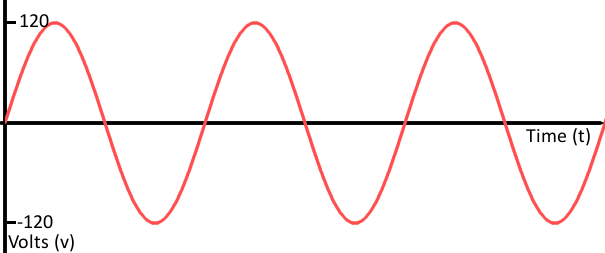
\includegraphics[width=\paperwidth/3]{Imagenes/analog.png}}
\caption{Gráfica representando una señal analógica.}
\end{figure}

\subsection*{Señales Digitales}
Una señal digital es una señal que se utiliza para representar datos como una secuencia de valores separados en cualquier momento. Solo puede tomar uno de un número fijo de valores. Este tipo de señal representa un número real dentro de un rango constante de valores.


\begin{figure}[ht!]
\makebox[\textwidth]{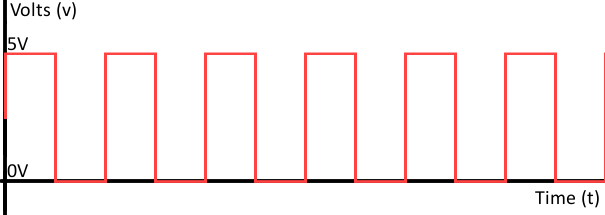
\includegraphics[width=\paperwidth/3]{Imagenes/digital.png}}
\caption{Gráfica representando una señal analógica.}
\end{figure}

\subsection*{Propiedades}
Las propiedades de las señales analógicas y digitales son las que las distinguen. Algunas propiedades se enumeran en la siguiente tabla:

\begin{figure}[ht!]
\makebox[\textwidth]{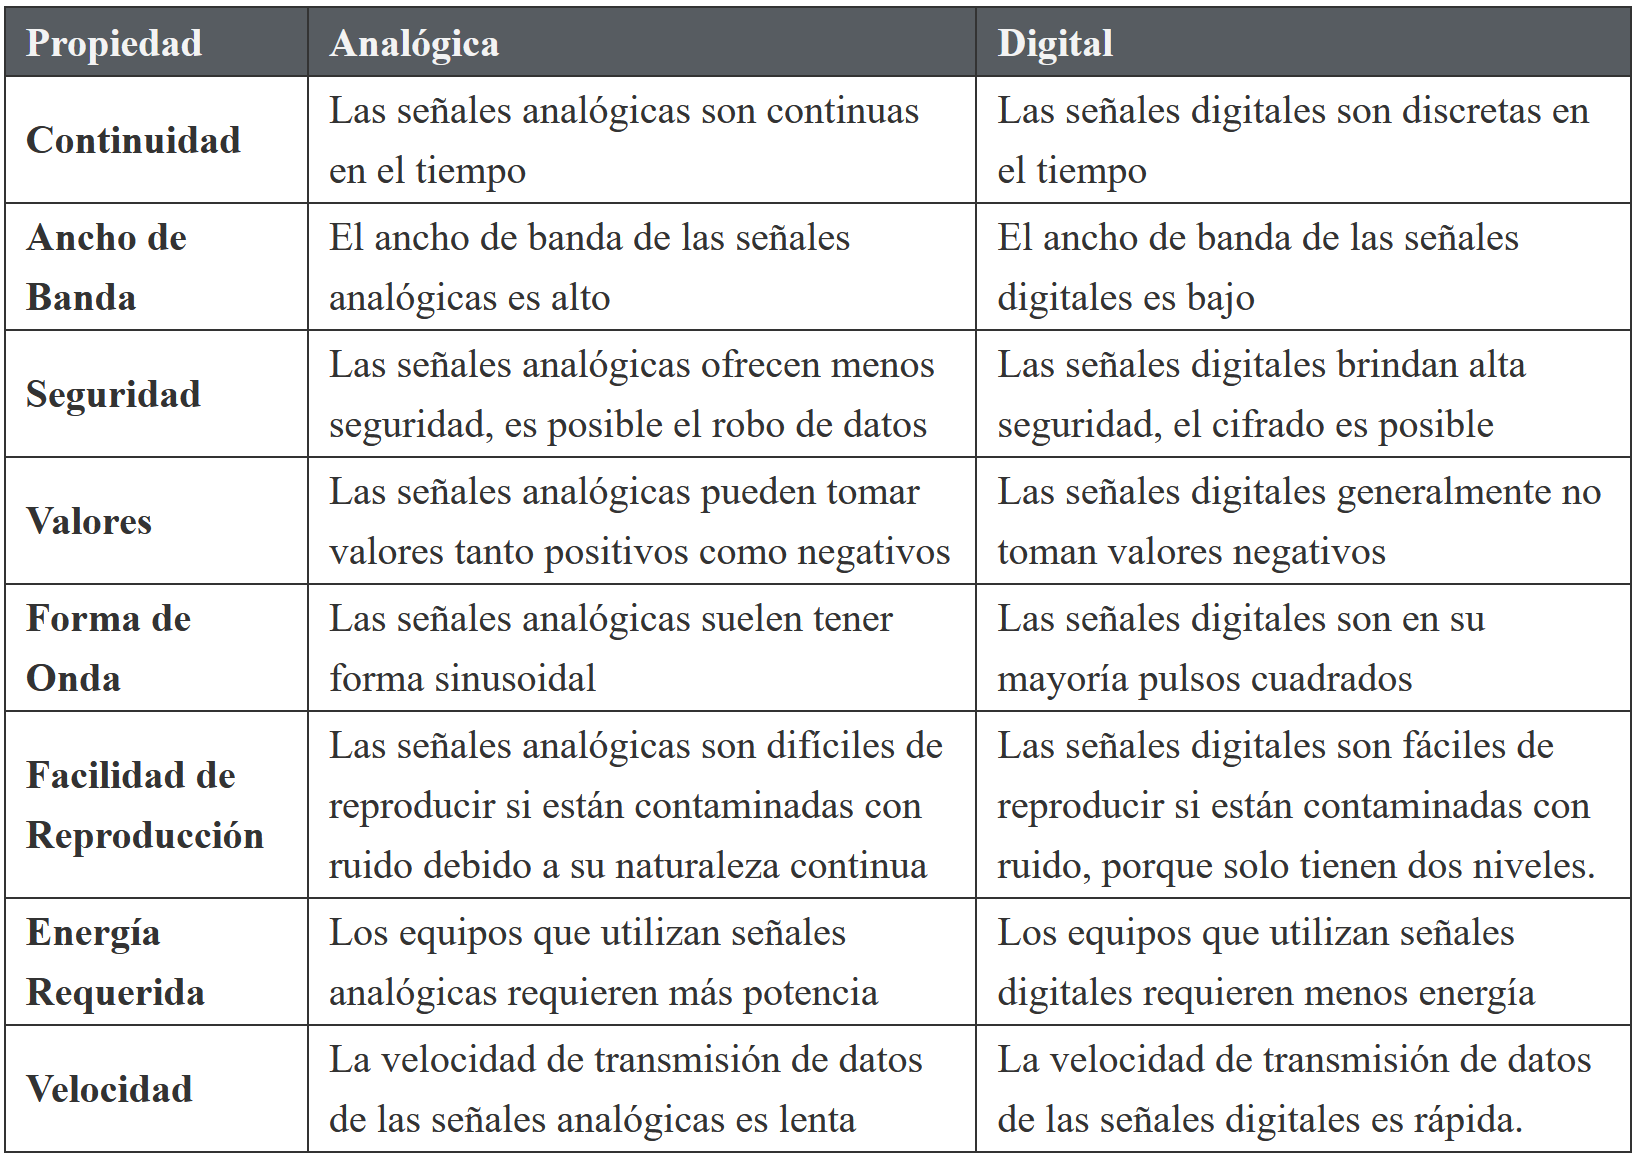
\includegraphics[width=\paperwidth/2]{Imagenes/tabla_digi_ana.png}}
\end{figure}

\subsection*{Equipo analógico frente a digital}
Muchos dispositivos vienen con funciones de traducción integradas de analógico a digital. Los micrófonos y los altavoces son ejemplos perfectos de dispositivos analógicos. \textit{La tecnología analógica} es más barata, pero existe una limitación en el tamaño de los datos que se pueden transmitir en un momento dado. \textit{La tecnología digital} ha revolucionado la forma en que funcionan la mayoría de los equipos. Los datos se convierten en código binario y luego se vuelven a ensamblar a su forma original en el punto de recepción. Dado que se pueden manipular fácilmente, ofrece una gama más amplia de opciones. El equipo digital es más caro que el equipo analógico. Los convertidores de analógico a digital (ADC) y los convertidores de digital a analógico (DAC) se utilizan para conectar dispositivos analógicos a digitales y viceversa. Estos convertidores se utilizan ampliamente en bloques de procesamiento de señales, como los que se utilizan en los sistemas de telecomunicaciones.
\subsection*{Calidad}
Cuando se habla de la calidad de una señal, lo primero que no interesa es el \textit{ruido}. \textit{¿Qué señal es más inmune al ruido?} Si se ve la forma de onda de la señal, se puede decir que las señales digitales son más inmunes al ruido. \textit{¿Por qué es así?}

Cuando el ruido golpea cualquier señal, cambia la forma de la onda en ese punto y para eliminar el ruido de la señal, es necesario producir una copia original de la señal. Ahora, considerando que el ruido se produce en una señal digital y distorsiona la forma de onda de tal manera que en un punto donde la señal tenía que estar en un nivel alto, está en algún lugar entre el nivel medio y alto. Por otro lado, si una señal analógica se distorsiona por el ruido, pasará desapercibida porque la señal ya es una serie de altibajos por lo que es difícil diferenciar la señal ruidosa de la original.

Entonces, podemos concluir que la calidad de las señales digitales es mejor que las señales analógicas debido a la inmunidad al ruido.
\subsubsection*{Aplicaciones}
La tecnología digital ha sido más eficiente en la industria de la telefonía celular. Los teléfonos analógicos se han vuelto redundantes a pesar de que la claridad y la calidad del sonido eran buenas. La tecnología analógica se compone de señales naturales como el habla humana. Con la tecnología digital, esta voz humana se puede guardar y almacenar en una computadora. Así, la tecnología digital abre el horizonte a un sinfín de posibles usos.
\item {\color{red}\textit{Conversión de una señal analógica a digital}}

Casi todos los parámetros ambientales medibles están en forma analógica como temperatura, sonido, presión, luz, etc. Estos datos no son posibles de almacenar con computadoras y procesadores digitales. Por lo tanto, este sistema necesita un dispositivo intermedio para convertir los datos de  analógicos en datos digitales para comunicarse con los procesadores digitales como microcontroladores y microprocesadores. El convertidor analógico a digital (ADC) es un circuito integrado electrónico que se utiliza para convertir las señales analógicas, como voltajes, a formato digital o binario que consta de 1 y 0. La mayoría de los ADC toman una entrada de voltaje de 0 a 10 V, de -5 V a + 5 V , etc. y, en consecuencia, produce una salida digital como una especie de número binario.

\begin{figure}[ht!]
\makebox[\textwidth]{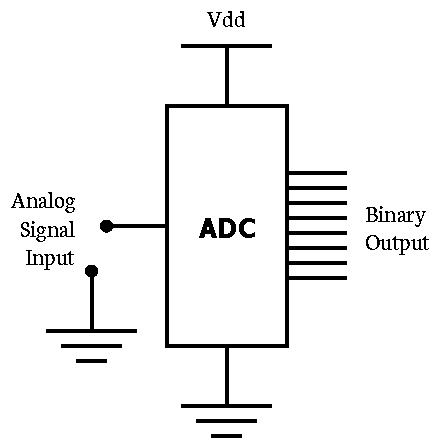
\includegraphics[width=\paperwidth/4]{Imagenes/adc.pdf}}
\caption{Esquema de un ADC}
\end{figure}
\subsubsection*{Proceso de conversión de analógico a digital}
El convertidor analógico a digital muestrea la señal analógica en cada flanco ascendente o descendente del reloj. En cada ciclo, el ADC obtiene la señal analógica, la mide y la convierte en un valor digital. El ADC convierte los datos de salida en una serie de valores digitales aproximando la señal con precisión arbitraria. En los ADC, dos factores determinan la precisión del valor digital que captura la señal analógica original. Estos son el nivel de cuantificación o la tasa de bits y la tasa de muestreo. La siguiente figura muestra cómo se realiza la conversión de analógico a digital. La tasa de bits decide la resolución\footnote{La resolución del ADC es el número de bits que utiliza para digitalizar las muestras de entrada. Para un ADC de n bits, el número de niveles digitales discretos que se pueden producir es $2n$.} de la salida digitalizada y puede observar en la siguiente figura dónde se utiliza ADC de 3 bits para convertir la señal analógica.
\begin{figure}[ht!]
\makebox[\textwidth]{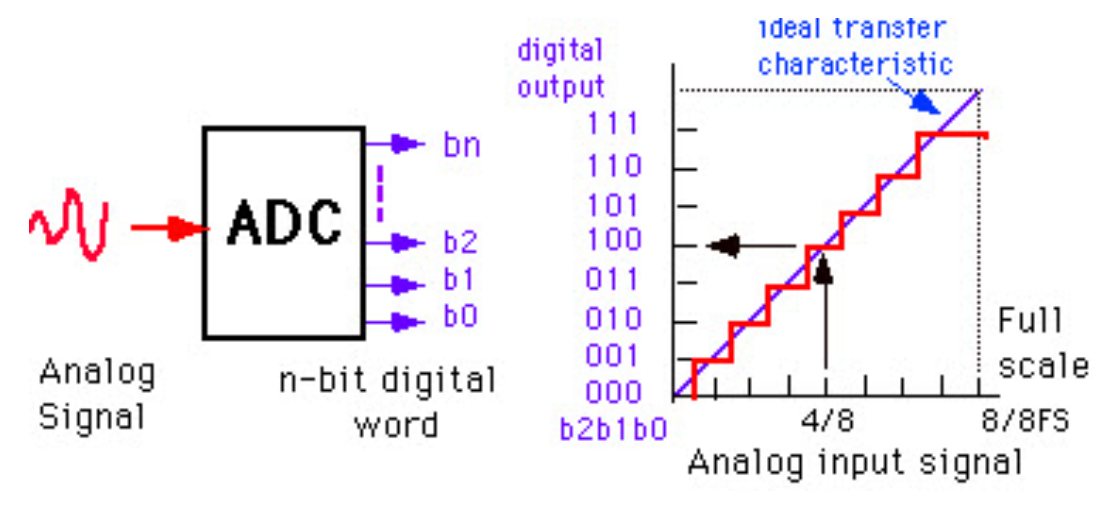
\includegraphics[width=\paperwidth*\real{0.4}]{Imagenes/process.png}}
\caption{Esquema de un ADC de 3 bits.}
\end{figure}

Otra consideración importante del ADC es la frecuencia de muestreo. El \textit{teorema de Nyquist-Shannon} establece que la reconstrucción de la señal adquirida introduce distorsión a menos que se muestree al menis dos veces la tasa del contenido de frecuencia más grande de la señal, como se puede observar en el diagrama: \\
\pagebreak
\begin{figure}[ht!]
\makebox[\textwidth]{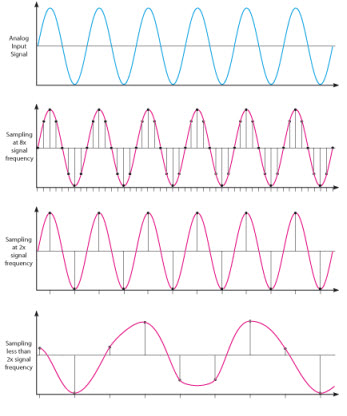
\includegraphics[width=\paperwidth*\real{0.33}]{Imagenes/nyq.jpg}}
\caption{Esquema de un ADC de 3 bits.}
\end{figure}

En el último caso sucede un fenómeno llamado \textbf{Aliasing} en el que una banda de alta frecuencia se superpone a una banda de baja frecuencia debido al cual no es posible la reconstrucción de la señal en el receptor.

\item {\color{red}\textit{Multiplexación analógica}}

La \textit{multiplexación es el proceso de combinar múltiples señales en una señal, a través de un medio compartido}. Si las señales analógicas se multiplexan, es multiplexación analógica y si las señales digitales se multiplexan, ese proceso es multiplexación digital.

\begin{figure}[ht!]
\makebox[\textwidth]{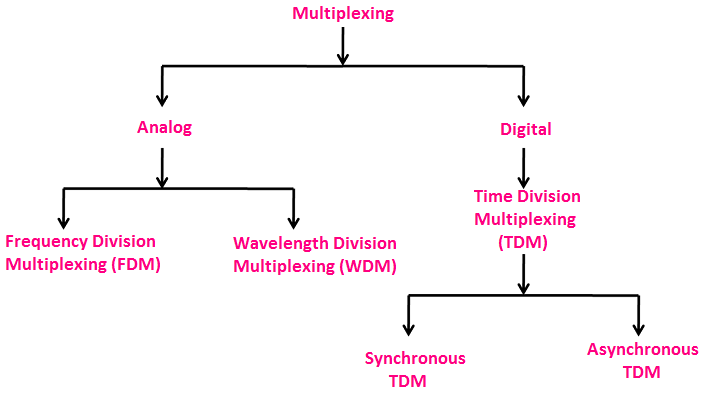
\includegraphics[width=\paperwidth*\real{0.4}]{Imagenes/multiplex.png}}
\caption{Tipos de multiplexación.}
\end{figure}

Las técnicas de multiplexación analógica involucran señales que son de naturaleza analógica. Las señales analógicas se multiplexan según su frecuencia (FDM: Frequency Division Multiplexing) o longitud de onda (WDM: Wavelength Division Multiplexing).

\begin{itemize}
\item \textbf{Frequency Division Multiplexing:} La multiplexación por división de frecuencia es una técnica analógica. Es la técnica de multiplexación más popular. Usamos esta técnica ampliamente en transmisión de radio y televisión. Esta técnica combina múltiples señales en una señal y se transmite a través del canal de comunicación. La multiplexación por división de frecuencia también se conoce como FDM. En esta técnica, el ancho de banda del canal de comunicación debería ser mayor que el ancho de banda combinado de las señales individuales.

\begin{figure}[ht!]
\makebox[\textwidth]{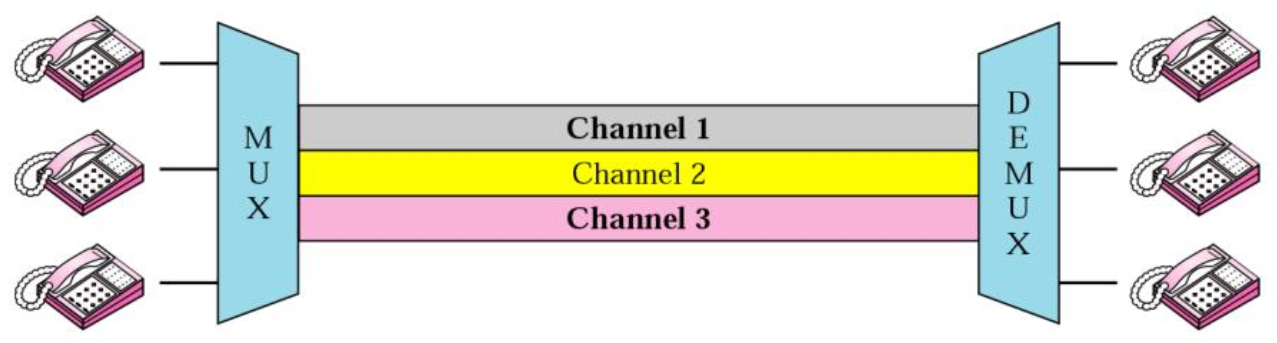
\includegraphics[width=\paperwidth*\real{0.4}]{Imagenes/fdm.png}}
\caption{Tipos de multiplexación.}
\end{figure}
\pagebreak
\item \textbf{Wavelenght Division Multiplexing:} La multiplexación por división de longitud de onda es una técnica analógica. Es el método más importante y más popular para aumentar la capacidad de una fibra óptica. Llongitud de onda y la frecuencia son inversamente proporcionales entre sí (es decir, una longitud de onda más larga significa baja frecuencia y una longitud de onda más corta significa alta frecuencia). Por lo tanto, el principio de funcionamiento de la multiplexación por división de longitud de onda es similar a la multiplexación por división de frecuencia. La única diferencia es que se utilizan señales ópticas de multiplexación por división de longitud de onda en lugar de señales eléctricas. En la multiplexación por división de longitud de onda, las señales ópticas se transmiten a través de cables de fibra óptica.
\end{itemize}
\item {\color{red}\textit{Digitalización de la voz}}

El proceso de codificación de voz permite transmitir y almacenar la señal de voz en forma digital eficientemente y sin pérdida de calidad. Desde el punto de vista de la transmisión de la señal de voz, la codificación de voz permite optimizar la utilización del canal de comunicación. Hay tres pasos en la digitalización de voz: 
\begin{enumerate}
\item \textbf{Sampling}

\item \textbf{Cuantificación}

\item  \textbf{Encoding}

\item \textbf{Compression (opcional)}
\end{enumerate}
\textbf{El muestreo} es el proceso de captura y grabación periódica de voz. El resultado del muestreo se denomina señal de modulación de amplitud de pulso (PAM\footnote{Pulse Amplitude Modulation}). La cuantificación es el proceso de asignar valores numéricos a la amplitud (altura o voltaje) de cada una de las muestras en la señal PAM utilizando una metodología de escala. La codificación es el proceso de representar el resultado de la cuantificación para cada muestra PAM en formato binario. Por ejemplo, cada muestra se puede expresar mediante un número binario de 8 bits, que puede tener 256 valores posibles. \\

Un método común para convertir una señal de voz analógica en una señal de voz digital es la modulación de código de pulso (PCM\footnote{Pulse Code Modulation}), que se basa en tomar 8000 muestras por segundo y codificar cada muestra con un número binario de 8 bits. Por tanto, PCM genera 64.000 bits por segundo (64 Kbps); no realiza compresión. \\

\textbf{La compresión}, el último paso para convertir una señal de voz analógica a digital, es opcional. El propósito de la compresión es reducir la cantidad de bits (voz digitalizada) que deben transmitirse por segundo con la menor cantidad posible de degradación de la calidad de la voz.

\begin{figure}[ht!]
\makebox[\textwidth]{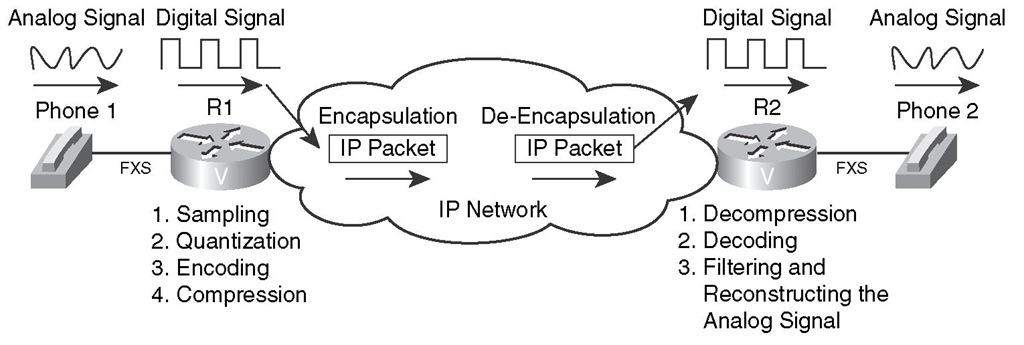
\includegraphics[width=\paperwidth*\real{0.5}]{Imagenes/ipenviada.jpg}}
\caption{En términos de redes se llevaría a cabo de acuerdo a este diagrama superficial.}
\end{figure}


\end{enumerate}


\begin{thebibliography}{9}
\bibitem{anadigi} 
Analog vs. Digital Signals fundaments. \href{https://solectroshop.com/en/blog/analog-vs-digital-signals-fundaments-n22}{https://solectroshop.com/en/blog/analog-vs-digital-signals-fundaments-n22} 6 de Junio, 2020

\bibitem{guru99} 
Analog vs Digital: What's the Difference?, \texttt{guru99.com} \href{https://www.guru99.com/analog-vs-digital.html\#7}{https://www.guru99.com/analog-vs-digital.html\#7}

\bibitem{diffen} 
Analog vs Digital \href{https://www.diffen.com/difference/Analog_vs_Digital}{https://www.diffen.com/difference/Analog_vs_Digital}

\bibitem{procus} 
How to Convert the Analog Signal to Digital Signal by ADC Converter \href{https://www.elprocus.com/analog-to-digital-adc-converter/}{https://www.elprocus.com/analog-to-digital-adc-converter/}

\bibitem{blogspot} 
Aliasing \href{http://communicationsystem4ru.blogspot.com/2016/03/aliasing.html}{http://communicationsystem4ru.blogspot.com/2016/03/aliasing.html}

\bibitem{tutorialspoint} 
What is Multiplexing and what are its types? \href{https://www.tutorialspoint.com/what-is-multiplexing-and-what-are-its-types}{https://www.tutorialspoint.com/what-is-multiplexing-and-what-are-its-types}


\bibitem{wwh} 
Digitizing and Packetizing Voice (Cisco VoIP Implementations) \href{http://what-when-how.com/ccnp-ont-exam-certification-guide/digitizing-and-packetizing-voice-cisco-voip-implementations/}{http://what-when-how.com/ccnp-ont-exam-certification-guide/digitizing-and-packetizing-voice-cisco-voip-implementations/}

\bibitem{wwh} 
Codificación de Voz y Audio \href{http://physionet.cps.unizar.es/~eduardo/investigacion/voz/coder.html}{http://physionet.cps.unizar.es/~eduardo/investigacion/voz/coder.html}

\end{thebibliography}
